\documentclass{article}

\usepackage{color}
\usepackage{listings}
\usepackage{graphicx}
\definecolor{MyYellow}{rgb}{1,1,0.8}
 
\lstset{language=Matlab,backgroundcolor=\color{MyYellow},basicstyle=\footnotesize,numberstyle=\footnotesize,numbers=left,stepnumber=1,numbersep=5pt,breaklines=true,frame=lines,tabsize=2}

\author{Ruurd Moelker \and Jan Paul Posma}
\date{\today}
\title{Signalen \& Systemen}

\begin{document}
\maketitle 

\section{Opgave 1}
Het tijdverschil tussen zender en ontvanger is de afstand gedeeld door de
snelheid van het geluid. De afstanden van de paden tot microfoon 1 en 2 geven
we respectiefelijk aan met $p_{1}$ en $p_{2}$. Met pythagoras kunnen $p_{1}$ en
$p_{2}$ berekend worden waarbij $Y_r$ en $X_v$ de korte zijden zijn voor
microfoon 1 en microfoon 2 $Y_{r}$ en $X_{v}-d$ heeft als zijden. Gegeven zijn de volgende
waarde: $$c = 333\frac{1}{3}$$ $$d = 0,4m$$ $$Y_{r} = 100m$$ Het relatieve
verschil in seconde van microfoon 1 en 2, respectiefelijk $t_1$ en $t_2$, wordt
gegeven met de volgende functies afhankelijk van $X_v$: $$t_{1}(X_{v}) =
\frac{p_{1}}{c}$$ $$t_{2}(X_{v}) = \frac{p_{2}}{c}$$ Waarbij: $$p_{1} =
\sqrt{X_{v}^{2} + Y_{r}^{2}}$$ $$p_{2} = \sqrt{(X_{v}-d)^{2} + Y_{r}^{2}}$$

\newpage
\section{Opgave 2}
De ontvangen signalen worden aangegeven met $x_{1}$ en $x_{2}$. In figuur
\ref{2a} staan drie periodes van de functies $x_{1}$ en $x_{2}$ waarbij $X_{v}
= 100m$:

$$x_{1}(t) = s(t - t_1)$$ $$x_{2}(t) = s(t - t_{2})$$ $$s(t) =
1000*sin(400*2\pi*t)$$


\begin{figure}[h]
	\center
	\begin{center}
	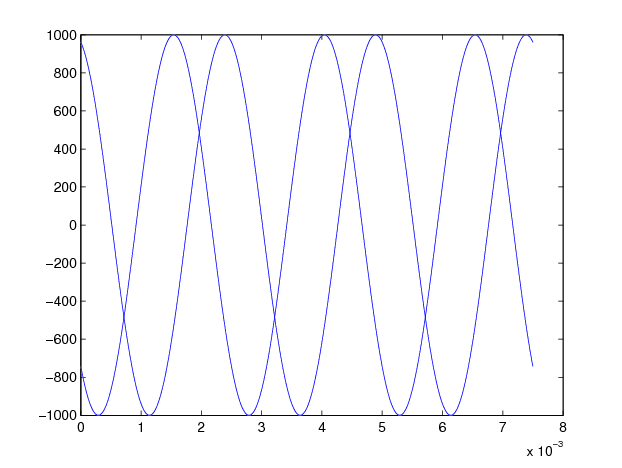
\includegraphics[width = 8cm]{2a.png}
	\caption{Plot twee ontvangen signalen}
	\end{center}
 \label{2a}
\end{figure}

If figuur \ref{2b} is ingezoomd op de dalen om zo het relatieve tijdverschil
tussen $x_1$ en $x_2$ te zien. Hieruit schatten wij dat er sprake is van een
relatieve tijdverschuiving van $8,5*10^4$ sec, deze komt
door het verschil van de dalen $3,65*10^{-3}$ en $2,8*10^{-3}$ te berekenen.

\begin{figure}[h]
	\begin{center}
	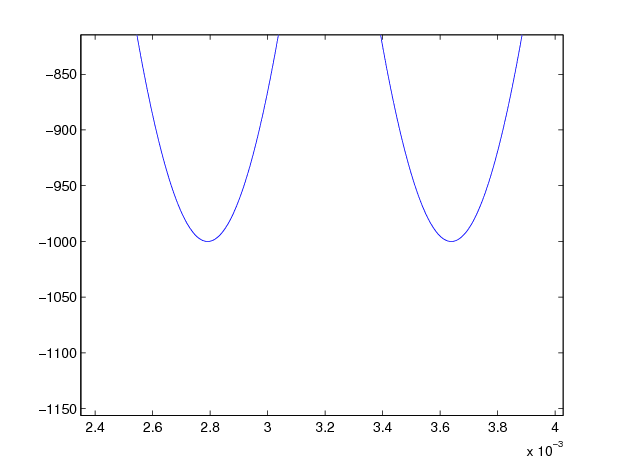
\includegraphics[width = 8cm]{2b.png}
	\caption{Plot ingezoomd op de dalen van de twee signalen}
	\end{center}
 \label{2b}
\end{figure}

\newpage
\section{Opgave 3}
De waarde van \begin{math}\varphi\end{math} hebben we bepaald door middel van het tijdverschil van de twee ontvangen signalen, gegeven het verschil berekend in de vorige opgave, volgens:
$$\varphi = sin^{-1}(\frac{d}{c} * (t_{1} - t_{2})) = 0,79 rad$$

Tevens hebben we $\varphi$ berekend met behulp van de meetkunde. Dit geeft:
$$tan^{-1} (\frac{X_{v}}{Y_{r}}) = 0,79rad$$

De gevonden waarde van $\varphi$ komen op twee significante cijfers overeen, dus de gebruikte methode blijkt te werken.

\section{Opgave 4}

De hoek tussen ontvanger en bron wordt berekend met de functie CalcDir. Deze functie verwacht twee complexe amplitudes die verkregen worden uit de geleverde functie DF\_Gen. De werking van de functie staat bij de code beschreven. 
\begin{lstlisting}
function [direction] = CalcDir(signal1, signal2)
%CALCDIR Calculates direction of the signals
%   given complex signals1 and 2, the direction is calculated by first
%   calculating de phase differences in rad. This is then converted to
%   seconds which is then used to calculate the direction. The direction is
%   returned in degrees.
    d = 0.4;
    ff = 400;
    ww = 2 * pi * ff;
    c = 1000/3;
    
    dfi = angle(signal1 .* conj(signal2));
    dt = dfi / ww;
    direction = real(asin(c/d*dt) * (180/pi));
end
\end{lstlisting}

Om het verschil in fase tussen de twee signalen te berekenen hebben we gebruik gemaakt van het feit dat $\Delta\varphi = angle\{X_{1}X_{2}^{*}\}$. Het bijbehorende bewijs staat hieronder gegeven.

$$X_{1} = A_{1}*e^{j\varphi_{1}}$$
$$X_{2} = A_{2}*e^{j\varphi_{2}}$$
$$angle\{X_{1}X_{2}^{*}\} = angle\{A_{1}*e^{j\varphi_{1}} * A_{2}*e^{-j\varphi_{2}}\}$$
$$= angle\{A_{1}*A_{2}*e^{j*(\varphi_{1}-\varphi_{2})}\}$$
$$= \varphi_{1}-\varphi_{2} = \Delta\varphi$$

\section{Opgave 5}

Het testen van onze functie hebben we gedaan door de methode TestDiff te maken. Deze methode staat hieronder uitgewerkt.

\begin{lstlisting}
function [] = TestDiff()
%TESTDIFF Plot DF_Gen theta vs our own calculated theta
%	901 samples are taken between -400 and 500 where our own calculated theta via the function CalcDir is compared to the theta from DF_Gen via a plot.
    x = -400:500;
    [X1, X2, originalTheta] = DF_gen(x);
    ourTheta = CalcDir(X1, X2);
    hold off;
    plot(x, originalTheta);
    hold on;
    plot(x, ourTheta);
    hold off;
end
\end{lstlisting}

De verkregen plot staat in figuur \ref{5a}. In de plot lijkt er sprake te zijn van een enkele lijn en dus precies gelijke waarden uit de twee functies. Echter is if figuur \ref{5b} te zien dat het wel degelijk gaat om twee verschillend gevonden hoeken.

\begin{figure}[h]
	\center
	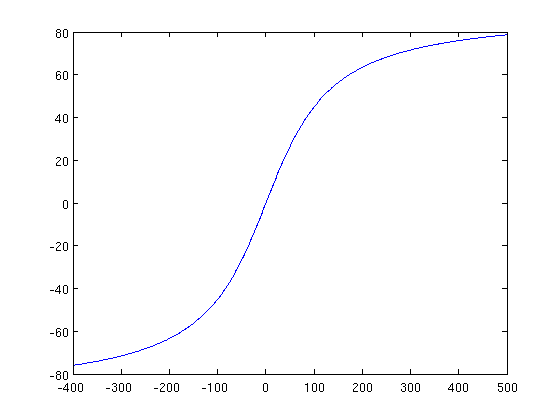
\includegraphics[width = 10cm]{5a.png}
	\caption{Plot gemaakt door functie TestDiff}
 \label{5a}
\end{figure}


\begin{figure}[h]
	\center
	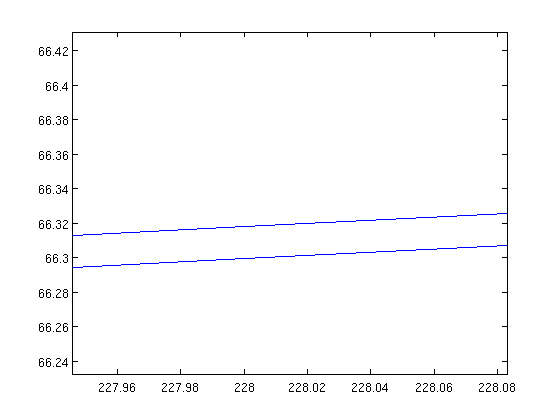
\includegraphics[width = 10cm]{5b.png}
	\caption{Plot waarbij de verschillende uitkomsten van de functies binnen TestDiff zichbaar zijn}
 \label{5b}	
\end{figure}

Hoewel er een verschil is tussen de echte theta en de gevonden theta volgens onze functie CalcDir is dit verschil dermate klein dat CalcDir een zeer betrouwbare geluidsrichting geeft.


\end{document}
